%% LyX 1.3 created this file.  For more info, see http://www.lyx.org/.
%% Do not edit unless you really know what you are doing.
\documentclass[english, 12pt]{article}
\usepackage{times}
%\usepackage{algorithm2e}
\usepackage{url}
\usepackage{bbm}
\usepackage[T1]{fontenc}
\usepackage[latin1]{inputenc}
\usepackage{geometry}
\geometry{verbose,letterpaper,tmargin=2cm,bmargin=2cm,lmargin=1.5cm,rmargin=1.5cm}
\usepackage{rotating}
\usepackage{color}
\usepackage{graphicx}
\usepackage{subcaption}
\usepackage{amsmath, amsthm, amssymb}
\usepackage{setspace}
\usepackage{lineno}
\usepackage{hyperref}
\usepackage{bbm}
\usepackage{makecell}

%\renewcommand{\arraystretch}{1.8}

\usepackage{xr}
\externaldocument{paper-ldpred2-supp}

%\linenumbers
%\doublespacing
\onehalfspacing
%\usepackage[authoryear]{natbib}
\usepackage{natbib} \bibpunct{(}{)}{;}{author-year}{}{,}

%Pour les rajouts
\usepackage{color}
\definecolor{trustcolor}{rgb}{0,0,1}

\usepackage{dsfont}
\usepackage[warn]{textcomp}
\usepackage{adjustbox}
\usepackage{multirow}
\usepackage{graphicx}
\graphicspath{{../figures/}}
\DeclareMathOperator*{\argmin}{\arg\!\min}

\let\tabbeg\tabular
\let\tabend\endtabular
\renewenvironment{tabular}{\begin{adjustbox}{max width=0.9\textwidth}\tabbeg}{\tabend\end{adjustbox}}

\makeatletter

%%%%%%%%%%%%%%%%%%%%%%%%%%%%%% LyX specific LaTeX commands.
%% Bold symbol macro for standard LaTeX users
%\newcommand{\boldsymbol}[1]{\mbox{\boldmath $#1$}}

%% Because html converters don't know tabularnewline
\providecommand{\tabularnewline}{\\}

\usepackage{babel}
\makeatother


\begin{document}


\title{LDpred2: better, faster, stronger}
\author{Florian Priv\'e,$^{\text{1,}*}$ Julyan Arbel,$^{\text{2}}$ and Bjarni J. Vilhj\'almsson$^{\text{1,}*}$}

\date{~ }
\maketitle

\noindent$^{\text{\sf 1}}$National Centre for Register-Based Research, Aarhus University, Aarhus, 8210, Denmark. \\
\noindent$^{\text{\sf 2}}$Univ.\ Grenoble Alpes, Inria, CNRS, Grenoble INP, LJK, Grenoble, 38000, France. \\
\noindent$^\ast$To whom correspondence should be addressed.\\

\noindent Contacts:
\begin{itemize}
\item \url{florian.prive.21@gmail.com}
\item \url{bjv@econ.au.dk}
\end{itemize}

\vspace*{4em}

\abstract{	

}


%%%%%%%%%%%%%%%%%%%%%%%%%%%%%%%%%%%%%%%%%%%%%%%%%%%%%%%%%%%%%%%%%%%%%%%%%%%%%%%%

\clearpage

\section{Introduction}

The use of polygenic scores (PGS) is widespread now.
There are high hopes for using these scores, which sum up the information of many genetic variants into a single score, into clinical practice. 
Predictive performance of PGS is inexorably bounded by heritability, the proportion of phenotypic variance that is attributable to genetics, so that their possibility of being used as a diagnostic tool for diseases is limited.
Nevertheless, it should be possible to use them to stratify the population into groups of different risk levels, to be able to identify individuals at high risk for a given disease [CITATION]. 
These people should then be monitored more closely to detect the disease and intervene sooner to maximize chances of remission (e.g.\ in the case of cancer).
PGS are also extensively used in epidemiology and economics as predictive variables of interest. For example, a recently derived PGS for education attainment has been the most predictive variable in social sciences so far [CITATION].

LDpred is a popular and powerful method for deriving polygenic scores based on summary statistics and a Linkage Disequilibrium (LD) matrix only \cite[]{vilhjalmsson2015modeling}.
It assumes there is a proportion $p$ of variants that are causal.
However, LDpred currently has several limitations that may result in limited predictive performance.
The non-infinitesimal version of LDpred, a Gibbs sampler, is particularly sensitive to model misspecification when applied to summary statistics with large sample sizes.
It may also be very unstable in long-range LD regions such as the human leukocyte antigen (HLA) region of chromosome 6. This issue has lead to the removal of this region from analyses  \cite[]{marquez2018modeling,lloyd2019improved}, which is a shame since this region of the genome contains several disease-associated variants, particularly with autoimmune diseases and psychiatric disorders [CITATIONS].
LDpred is also considered not particularly fast, nor memory-efficient, nor it provides truly sparse models as in its model specification.

Here, we present LDpred2, a new version of LDpred, that aims to cope with the issues presented before.
We provide a faster and more robust implementation of LDpred in R package bigsnpr \cite[]{prive2017efficient}.
We also provide two new options: a ``sparse'' option, where LDpred2 truly fit some effects to be zero, therefore providing a sparse vector of effects; and an ``auto'' option, where LDpred2 automatically estimates the sparsity $p$ and the (SNP) heritability $h^2$, therefore for which there is no need for validation data to choose hyper-parameters performing best.
We show that [DESCRIBE RESULTS].


%%%%%%%%%%%%%%%%%%%%%%%%%%%%%%%%%%%%%%%%%%%%%%%%%%%%%%%%%%%%%%%%%%%%%%%%%%%%%%%%

\section{Results}

\subsection*{Overview of methods}

Here we present LDpred2, a new version of LDpred \cite[]{vilhjalmsson2015modeling}.
LDpred2 has 4 options: 1) LDpred2-inf, an infinitesimal model similar to the one in LDpred1; 2) LDpred2-grid (or simply LDpred2) that is the main LDpred model, where a grid of values for hyper-parameters $p$ (the proportion of causal variants) and $h^2$ (the SNP heritability) are tuned using a validation test; 3) LDpred3-sparse, which is similar to LDpred2-grid but where effects can be exactly 0, offering a truly sparse version of LDpred; 4) LDpred2-auto, which automatically estimate $p$ and $h^2$ and therefore is free of hyper-parameter to optimize.
As a recall, LDpred1 has two options: LDpred1-inf and LDpred1-grid, where only $p$ is optimized.

We compare the two versions of LDpred using 6 simulation scenarios to understand in which cases it is important to use the new version. We also compare these two versions in 8 binary phenotypes of major interest using published external summary statistics and the UK Biobank data.

\subsection*{Simulations}

Figure \ref{fig:AUC-simu} presents the simulation results comparing LDpred1 (v1.0.0 as implemented by \cite{vilhjalmsson2015modeling}) with the new LDpred2 (as implemented in R package bigsnpr). 
6 simulation scenarios are used, each repeated 10 times.
In the first 4 simulations scenarios, a heritability of 40\% and a prevalence of 15\% are used. We simulate 300, 3000, 30,000 or 300,000 causal variants anywhere on the genome. 
In these scenarios, infinitesimal models are performing similarly. When testing a grid of parameters, LDpred2 performed substantially better than LDpred1 in the cases where the number of causal variations is smaller, i.e.\ in the case of 300 or 3000 causal variants ($p$=2.5e-4 and 2.5e-3). For example, in simulations with 300 causal variants, AUC of 73.5\% is obtained with LDpred1 while an AUC of 81.9\% is obtained with LDpred2.
In these scenarios, all 3 non-infinitesimal models of LDpred2 perform equally well.
In HLA scenarios, i.e.\ where causal variants are sampled in a region with variants at high LD, LDpred1 perform poorly. In these HLA scenarios, all LDpred2 models perform well, although LDpred2-auto perform slightly worse than other models.

%% FIGURE 1 HERE
\begin{figure}[h]
\centerline{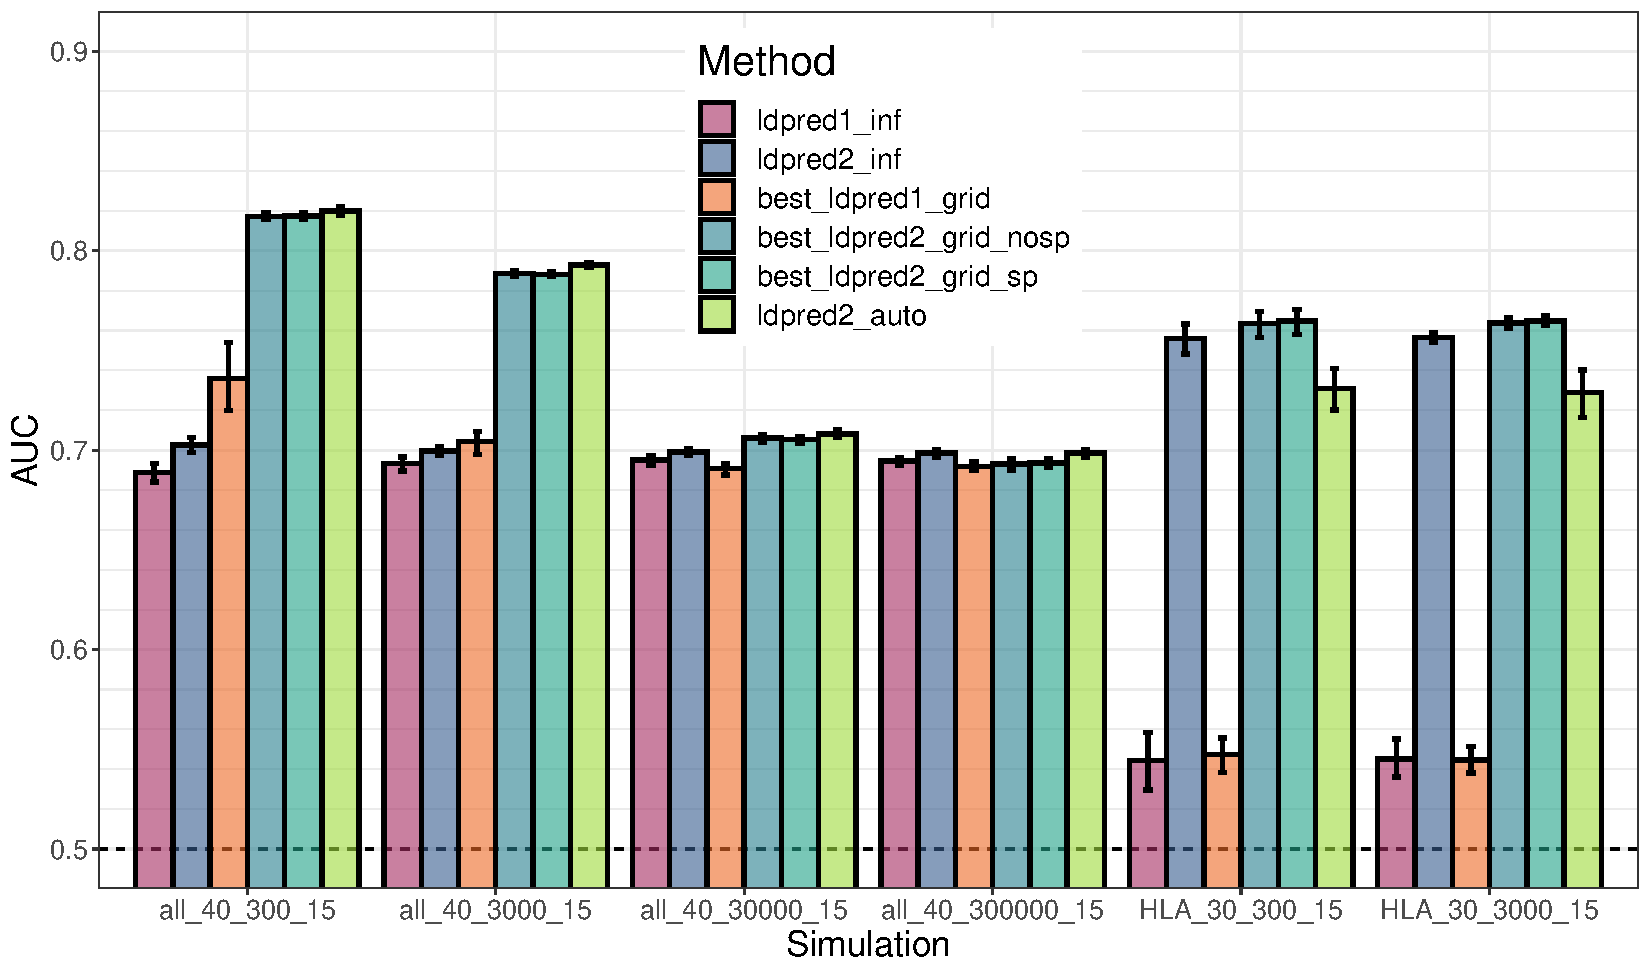
\includegraphics[width=0.95\textwidth]{AUC-simu}}
\caption{Results of the 6 simulation scenarios. 
Scenarios are named with 4 parts, separated by underscore: 1) ``all'' means that causal variants were randomly sampled anywhere on the genome while ``HLA'' means that they were sampled in the HLA region of chromosome 6 (25-35 Mb); 2) the heritability (in \%); 3) the number of causal variants; 4) the prevalence (in \%).
Bars present the mean and 95\% CI of $10^4$ non-parametric bootstrap replicates of the mean AUC of 10 simulations for each scenario. 
%See corresponding values in table S1.
}
\label{fig:AUC-simu}
\end{figure}

\subsection*{Real data}

Figure \ref{fig:AUC-real} presents the results of real data applications comparing LDpred1 (v1.0.0 as implemented by \cite{vilhjalmsson2015modeling}) with the new LDpred2 (as implemented in R package bigsnpr). 
8 binary phenotypes are used, summarized in table \ref{tab:sumstats}.
For T1D, T2D, BRCA, PRCA and MDD, all LDpred2 models perform much better than LDpred1. For example, for BRCA, AUC improves from 58.5\% with LDpred1 to 65\% with LDpred2, and from 55\% to 75\% for T1D. 
For Asthma, CAD and RA, predictive performances of LDpred1 and LDpred2 are similar.

As in simulations, the sparse version of LDpred2 performs equally well as the original version, with the exception of PRCA, for which it performs poorly.
For CAD, PRCA and TD1, LDpred2-auto perform much worse than LDpred2, otherwise it performs similarly.

%% FIGURE 2 HERE
\begin{figure}[h]
\centerline{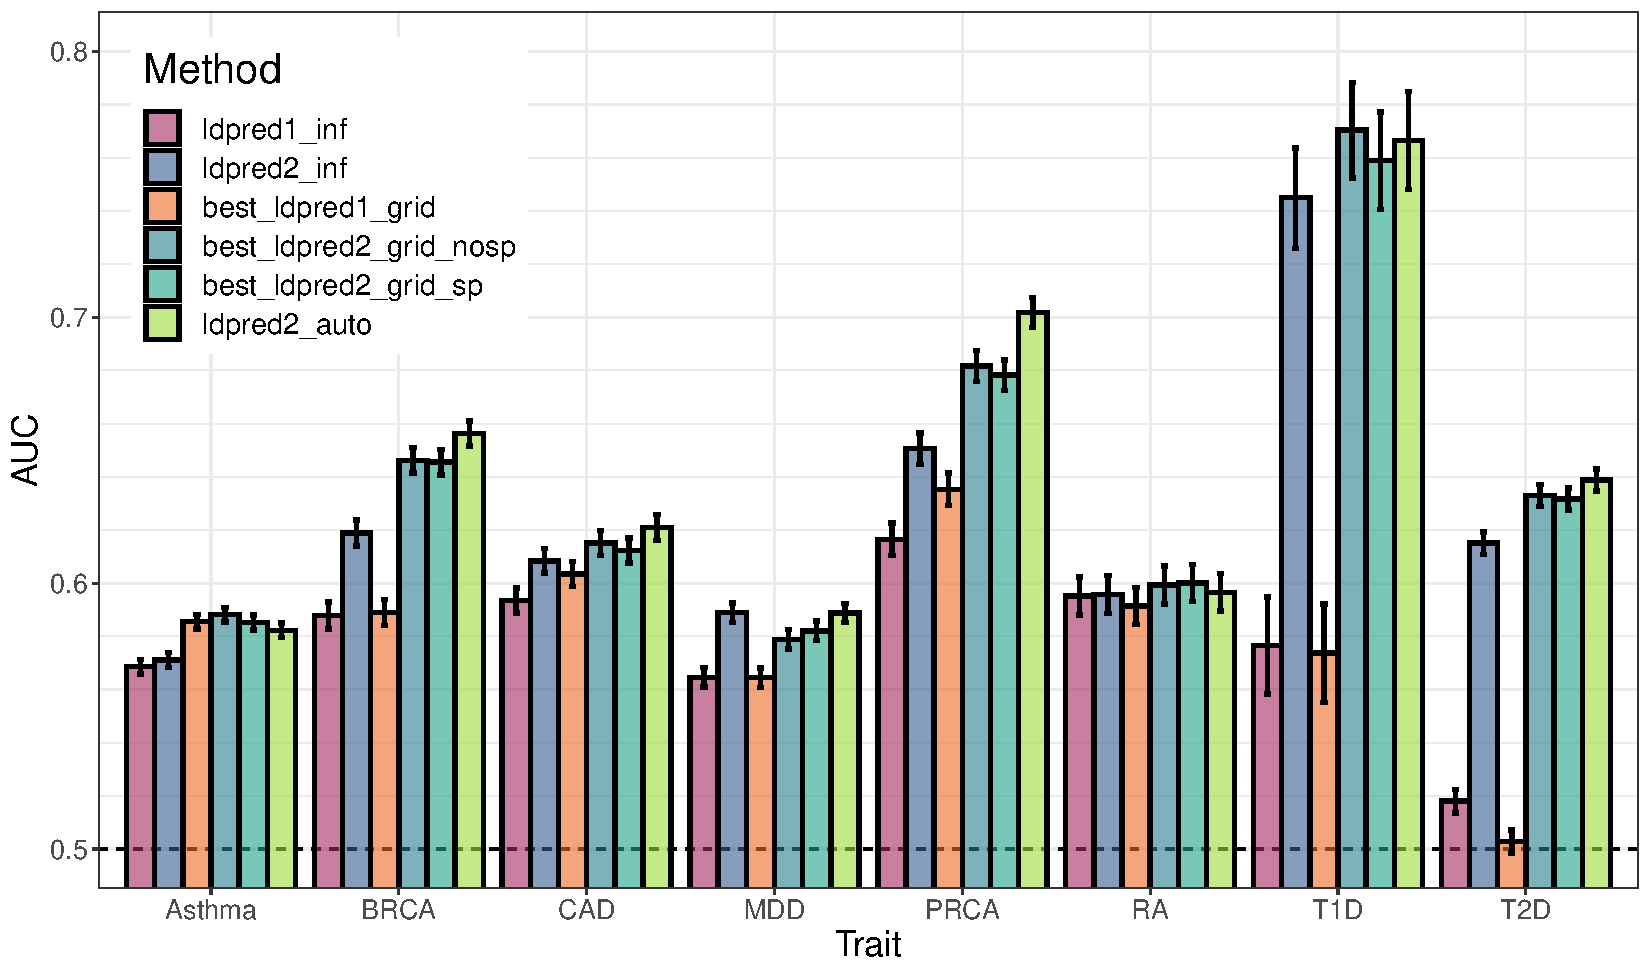
\includegraphics[width=0.85\textwidth]{AUC-real}}
\caption{Results of the real data applications using published external summary statistics.
Bars present AUC values on the test set of UKBB (mean and 95\% CI from $10^4$ bootstrap samples).
%See corresponding values in table S2.
}
\label{fig:AUC-real}
\end{figure}

%%%%%%%%%%%%%%%%%%%%%%%%%%%%%%%%%%%%%%%%%%%%%%%%%%%%%%%%%%%%%%%%%%%%%%%%%%%%%%%%

\section{Discussion}

Here we present LDpred2, a new version of LDpred. 
LDpred is widely used and has the potential to provide polygenic models with good predictive performance \cite{khera2018genome}. 
Yet, it has some instability issues.
We propose a new version to solve these instability issues and try to improve other points as well.

We show that LDpred2 is much more stable and provides higher prediction than LDpred1.
We demonstrate that LDpred1 has some large issues due to long-range LD regions such as the HLA region.
Indeed, both LDpred1 and LDpred1-inf perform poorly in the simulations where causal variants are the HLA region.
In constrast, LDpred2 perform very well. We hypothesize that LDpred1 does not use a window size that is large enough to account for long-range LD such as in the HLA region.
In LDpred2, we use a window size of 3 cM, which is much larger and enable LDpred2 to work well even when causal variants are in long-range LD regions.
We hypothesize that using a larger LD window explains the 5 real traits where LDpred2 performs much better than LDpred1, especially because LDpred2-inf performs better than LDpred1-inf.
We strongly discourage against removing these regions as suggested by others as these regions, especially the HLA region, contain lots of variants associated with many traits such as autoimmune diseases and psychiatric disorders, and are therefore very useful for prediction.

In LDpred2, we also test more values for $p$ (17 instead of 7 by default) and for $h^2$ (3 instead of 1).
When testing the grid of hyper-parameters of $p$ and $h2$, we also allow for testing an option to enable sparse models in LDpred2 (see after).
Overall, we test a grid of 102 different values in LDpred2 instead of 7 in LDpred1, we use 5 times as many iterations, use a larger window size for computing correlation, yet it is LDpred2 is still faster than LDpred1.
LDpred2 is faster than LDpred1 because we provide a very efficient parallel implementation in C++. The parallelization is performed on the grid of parameters, but can also be performed chromosome-wise, as each chromosome is processed independently in LDpred2 (see methods).
As an example, it takes less than two hours to run LDpred2-inf, LDpred2-grid (108 hyper-parameters values) and LDpred2-auto for a chromosome with 100K variants and using 8 cores, and only 15 minutes for a chromosome with 20K variants.
Pre-computing the LD matrix for a chromosome with 100K variants takes 11 minutes using 16 cores.

LDpred2 also comes with two new models.
When the sparse option is enabled, it provide models that are truly sparse, as compared to LDpred1 which outputs very small non-zero effect sizes \cite{cecile2019polygenic}.
It can provide sparse effect sizes as much as 98\% for small $p$, while keeping predictive performance as good non-sparse models, as opposed to if very small effects were simply discarded \cite[]{bolli2019software}.
This sparse model perform equally well as the non-sparse model, therefore we encourage users to test it in the grid and to choose it if it performs equally well as the non-sparse model.
As for LDpred2-auto, which automatically estimates values for hyper-parameters $p$ and $h^2$, it performs equally well as other LDpred2 models in simulations, but does not perform well for half of the real traits analyzed here.
More investigations need to perform to understand the poor results of LDpred2-auto for some real traits.




%%%%%%%%%%%%%%%%%%%%%%%%%%%%%%%%%%%%%%%%%%%%%%%%%%%%%%%%%%%%%%%%%%%%%%%%%%%%%%%%

\section{Methods}

\subsection*{Simulation analyses}

We use the UK Biobank data for both real data analyses and simulations. We restrict individuals to White-British individuals used in the PC computation of the UK Biobank (i.e.\ unrelated and quality-controlled). We restrict variants to HapMap3 variants.
This results in 337,475 individuals and 1,194,574 variants.
We use 10,000 individuals as a validation set for choosing optimal hyper-parameters and computing correlations between variants (LD matrix). 
We use 300,000 other individuals for running logistic GWAS to create summary statistics.
We use the remaining 27,475 individuals as test set for evaluating models.

We simulate binary phenotypes with a heritability of $h^2 = 0.4$ (or 0.3)  using a Liability Threshold Model (LTM) with a prevalence of 15\% \cite[]{falconer1965inheritance}. 
We vary the number of causal variants (300, 3000, 30K, or 300K) to match a range of genetic architectures from low to high polygenicity.
Liability scores are computed from a model with additive effects only: we compute the liability score of the i-th individual as \(y_i = \sum_{j\in S_\text{causal}} w_j \widetilde{G_{i,j}} + \epsilon_i,\) where $S_\text{causal}$ is the set of causal variants, $w_j$ are weights generated from a Gaussian distribution $N(0, h^2 / \vert S_\text{causal} \vert)$, $G_{i,j}$ is the allele count of individual $i$ for variant $j$, $\widetilde{G_{i,j}}$ corresponds to its standardized version (zero mean and unit variance), and $\epsilon$ follows a Gaussian distribution $N(0, 1 - h^2)$.
Causal variants are chosen randomly anywhere on the genome. 
We make two other simulation scenarios with 300 or 3000 causal variants randomly chosen in the HLA region (chromosome 6, 25-35 Mb).
Both parts of the $y_i$ are scaled such that the variance of the genetic liability is exactly $h^2$ and the variance of the total liability is exactly $1$. 
This is implemented in function \texttt{snp\_simuPheno} of R package bigsnpr.
Each simulation scenario is repeated 10 times and averages of the Area Under the ROC Curve (AUC) are reported. 


\subsection*{Real data analyses}

We use the same data as in the simulation analyses. We use the same 10,000 individuals as validation set, and use the remaining 327,475 individuals as test set.
We use external published GWAS summary statistics listed in table \ref{tab:sumstats}.
We defined phenotypes as done in \cite{prive2019making}. For details, please refer to our R code (Software and code availability section).

%% TABLE 1 HERE
\begin{table}[h]
	\centering
	\begin{tabular}{|l|c|c|c|c|}
		\hline
		Trait & GWAS citation & GWAS sample size & GWAS \#variants \\
		\hline
		Breast cancer (BRCA) & \cite{michailidou2017association} & 137,045 / 119,078 & 11,792,542 \\
		Rheumatoid arthritis (RA) & \cite{okada2014genetics} & ~~29,880 / ~~73,758 & ~~9,739,303 \\
		Type 1 diabetes (T1D) & \cite{censin2017childhood} & ~~~~~5913 / ~~~~~8828  & ~~8,996,866 \\
		Type 2 diabetes (T2D) & \cite{scott2017expanded} & ~~26,676 / 132,532 & 12,056,346 \\
		Prostate cancer (PRCA) & \cite{schumacher2018association} & ~~79,148 / ~~61,106 & 20,370,946 \\
		Depression (MDD) & \cite{wray2018genome} & ~~59,851 / 113,154 & 13,554,550 \\
		Coronary artery disease (CAD) & \cite{nikpay2015comprehensive} & ~~60,801 / 123,504 & ~~9,455,778 \\
		Asthma & \cite{demenais2018multiancestry} & ~~19,954 / 107,715 & ~~2,001,280 \\
		\hline
	\end{tabular}
	\caption{Summary of external GWAS summary statistics used. The GWAS sample size is the number of cases / controls in the GWAS. \label{tab:sumstats}}
\end{table}


\subsection*{From marginal effects to joint effects}

In this section, we explain how we can obtain joint effects from summary statistics (marginal effects) and a correlation matrix.
Let us denote by $S$ the diagonal matrix with standard deviations of the $p$ variants, $C_n = I_n - 1 1^T / n$ the centering matrix, $G$ the genotype matrix of $n$ individuals and $p$ variants, and $y$ the phenotype vector for $n$ individuals.
Then, the marginal effects (assuming no other covariates than the intercept) are given by 
\[\hat{\beta}_{marg} = S^{-2} G^T C_n y ~,\]
while the joint effects are obtained by solving
\[\begin{bmatrix} \hat{\alpha} \\ \hat{\beta}_{joint} \end{bmatrix} = \left(\begin{bmatrix} 1 & G \end{bmatrix}^T \begin{bmatrix} 1 & G \end{bmatrix}\right)^{-1} \begin{bmatrix} 1 & G \end{bmatrix}^T y ~.\]
Using the Woodburry formula, we get 
\[\hat{\beta}_{joint} = (G^T C_n G)^{-1} G^T C_n y ~.\]
We further note that the correlation matrix of $G$ is \(K =  S^{-1} G^T C_n G  S^{-1}\).
Then we get $\hat{\beta}_{joint} = S^{-1} K^{-1} S \hat{\beta}_{marg}$.

For one marginal effect $\hat{\beta}$, let us denote by $y^*$ and $g^*$ the corresponding phenotype and genotype (residualized from $K$ covariates, e.g.\ centering them).
Then,
$\text{var}(\hat{\beta}) = \dfrac{(y^* - \hat{\beta} g^*)^T (y^* - \hat{\beta} g^*)}{(N - K - 1) ~ g^{*T} g^*} \approx \dfrac{y^{*T} y^*}{N ~ g^{*T} g^*} \approx \dfrac{\text{var}(y)}{N ~ \text{var}(g)}$.
Thus, we can derive $\text{sd}(g) \approx \dfrac{\text{sd}(y)}{\text{sd}(\hat{\beta}) ~ \sqrt{N}}$ and $\left(\text{sd}(g) ~ \hat{\beta}\right) \approx \dfrac{\hat{\beta}}{\text{sd}(\hat{\beta})} \dfrac{\text{sd}(y)}{\sqrt{N}}$.

Let us go back to the formula we derived before: $\hat{\beta}_{joint} = S^{-1} K^{-1} S \hat{\beta}_{marg}$. As $\text{sd}(y)$ is the same for all variants, it is cancelled out by $S^{-1}$ and $S$. Then it justifies the use of Z-scores ($\hat{\beta} / \text{sd}(\hat{\beta})$) divided by $\sqrt{N}$ as input for LDpred. Then, the effect sizes that LDpred outputs need to be scaled by multiplying by $\left(\text{sd}(\hat{\beta}) ~ \sqrt{N}\right)$.
Note that LDpred (v1) and other similar methods scale the output dividing by the standard deviation of genotypes. This is correct when $\text{sd}(y) = 1$ only.



\subsection*{Overview of LDpred model}

LDpred assumes the following model for effect sizes,
\begin{equation}\label{eq:model}
\beta_j \sim \left\{
\begin{array}{ll}
\mathcal N\left(0, \dfrac{h^2}{M p}\right) & \mbox{with probably $p$,} \\
0 & \mbox{otherwise,}
\end{array}
\right.
\end{equation}
where $p$ is the proportion of causal variants, $M$ the number of variants and $h^2$ the (SNP) heritability.
\cite{vilhjalmsson2015modeling} estimates $h^2$ using constrained LD score regression (intercept fixed to 1) and recommend testing a grid of hyper-parameter values for $p$ (e.g.\ 1, 0.3, 0.1, 0.03, 0.01, etc.).

\newcommand{\hmpn}{\dfrac{h^2}{M p} + \dfrac{1}{N}}
\newcommand{\phmpn}{\dfrac{p}{\sqrt{\hmpn}}}
\newcommand{\betahmpn}{\dfrac{\tilde{\beta}_j^2}{\hmpn}}

To estimate effect sizes $\beta_j$, \cite{vilhjalmsson2015modeling} use a Gibbs sampler [REALLY A GS?]. They compute the probability that variant $j$ is causal as 
\[\bar{p}_j = P\left(\beta_j \sim \mathcal N(\cdot,\cdot) ~|~ \tilde{\beta}_j\right) = \dfrac{\phmpn \exp\left\lbrace-\dfrac{1}{2} \betahmpn\right\rbrace}{\phmpn \exp\left\lbrace-\dfrac{1}{2} \betahmpn\right\rbrace + \dfrac{1-p}{\sqrt{\dfrac{1}{N}}} \exp\left\lbrace-\dfrac{1}{2} \dfrac{\tilde{\beta}_j^2}{\dfrac{1}{N}}\right\rbrace}~,\]
which we rewrite as
\begin{equation}
\bar{p}_j = \dfrac{1}{1 + \dfrac{1-p}{p} \sqrt{1 + \dfrac{N h^2}{Mp}} \exp\left\lbrace-\dfrac{1}{2} \dfrac{N \tilde{\beta}_j^2}{1 + \dfrac{Mp}{N h^2}}\right\rbrace}~.
\end{equation}

Then, $\beta_j$ is sampled according to
\begin{equation}\label{eg:beta_random}
\beta_j ~|~ \tilde{\beta}_j \sim \left\{
\begin{array}{ll}
\mathcal N\left(\dfrac{1}{1 + \dfrac{M p}{N h^2}} \tilde{\beta}_j, \dfrac{1}{1 + \dfrac{M p}{N h^2}}\dfrac{1}{N}\right) & \mbox{with probably $\bar{p}_j$,} \\
0 & \mbox{otherwise.}
\end{array}
\right.
\end{equation}

[TO COMPLETE + CLEARER -> SHOULD SHOW THAT IT IS ITERATIVE]

\subsection*{New LDpred2 models}

LDpred2 comes with two extensions of the LDpred model.

The first extension consists in estimating $p$ and $h^2$ in the model, as opposed to testing several values of $p$ and estimating $h2$ using constrained LD score regression \cite[]{bulik2015ld}. This makes LDpred2-auto a method free of hyper-parameters which can therefore directly be applied to data without the need of a validation dataset to choose best-performing hyper-parameters.
To estimate $p$, we count the number of causal variants (i.e.\ $S = \sum_j(\beta_j \neq 0)$ in equation \ref{eg:beta_random}). 
We can assume that $S \sim B(M, p)$, so if we place a prior $p \sim \text{Beta}(1, 1) \equiv \mathcal{U}(0, 1)$, we can sample $p$ from the conjugate prior $p \sim \text{Beta}(1 + S, 1 + M - S)$.
Due to complexity reasons, we could not derive a Bayesian estimator of $h^2$. Instead, we estimate $h^2 = \beta^T K \beta$, where $K$ is the correlation matrix.

The second extension, LDpred2-sparse, aims at providing sparse effect size estimates, i.e. that some resulting effects are exactly 0.
When the sparse solution is sought and when $\bar{p}_j < p$, we set $\beta_j = 0$.
Note that LDpred2-auto does not have a sparse option, but it is possible to run LDpred2-sparse with the $p$ and $h^2$ estimates from LDpred2-auto.

\subsection*{New strategy for local correlation}

LDpred has a window size parameter that needs to be set; for a given variant, correlations with other variants outside of this window are assumed to be 0.
The recommended value for this window (in number of variants) is to use the total number of variants divided by 3000, which corresponds to a window radius of around 2 Mb \cite[]{vilhjalmsson2015modeling}.
After investigating, we come to the conclusion that this window size is not large enough. Indeed, the human leukocyte antigen (HLA) region of chromosome 6 is 8 Mb long \cite[]{price2008long}. 
Using a window of 8Mb would be computationally and memory inefficient.
Instead, we propose to use genetic distances. Genome-wide, 1 Mb corresponds on average to 1 cM. Yet, the HLA region is only 3 cM long (vs.\ 8 Mb long).
Therefore, genetic distances enable to capture the same LD using a globally smaller window.
We provide function \texttt{snp\_asGeneticPos()} in package bignspr to easily interpolate physical position to genetic positions.
We recommend to use genetic positions and to use a size parameter of 3 cM when computing the correlation between variants for LDpred2. 
Note that, in the code, we use \texttt{size = 3 / 1000} as parameter \texttt{size} is internally multiplied by 1000 in functions of package bigsnpr.

\subsection*{New strategy for running LDpred2}

We recommend to run LDpred2 per chromosome.
Even if it is possible to run LDpred2 genome-wide, this approach has two limitations. First, it can be memory and computationally demanding to do so. For around one million (1M) variants, storing the 1M$\times$1M sparse correlation matrix takes more than 32 GB of memory. 
Doubling to 2M variants would require 128 GB of RAM to store the matrix.
Second, as noted in \cite{prive2019making}, it may be beneficial to assume that architecture of traits may be different for different chromosomes.
For example, autoimmune diseases clearly show larger effects on chromosome 6. compared to other chromosomes.
Assuming the same model for genetic effects genome-wide could results in severe model misspecification, which would lead to suboptimal predictive performance.
Moreover, since the inverse of a block-diagonal matrix is formed from the inverse of each block, it should be safe to run LDpred2 for each chromosome and then combining the results.  


%%%%%%%%%%%%%%%%%%%%%%%%%%%%%%%%%%%%%%%%%%%%%%%%%%%%%%%%%%%%%%%%%%%%%%%%%%%%%%%%

\clearpage
%\vspace*{5em}

\section*{Software and code availability}

All code used for this paper is available at \url{https://github.com/privefl/paper-ldpred2/tree/master/code}.
R package bigsnpr can be installed from either CRAN or GitHub (see \url{https://github.com/privefl/bigsnpr}).
A tutorial on the steps to run LDpred2 using some small example data is available at \url{https://privefl.github.io/bigsnpr/articles/LDpred2.html}. 

\section*{Acknowledgements}

This research has been conducted using the UK Biobank Resource under Application Number 41181.

F.P. and B.V.\ are supported by the Danish National Research Foundation (Niels Bohr Professorship to Prof. John McGrath), and also acknowledge the Lundbeck Foundation Initiative for Integrative Psychiatric Research, iPSYCH (R248-2017-2003).

\section*{Declaration of Interests}

The authors declare no competing interests.

%%%%%%%%%%%%%%%%%%%%%%%%%%%%%%%%%%%%%%%%%%%%%%%%%%%%%%%%%%%%%%%%%%%%%%%%%%%%%%%%

\clearpage

\bibliographystyle{natbib}
\bibliography{refs}

%%%%%%%%%%%%%%%%%%%%%%%%%%%%%%%%%%%%%%%%%%%%%%%%%%%%%%%%%%%%%%%%%%%%%%%%%%%%%%%%

\end{document}
